\documentclass[xcolor=table,10pt,final]{beamer}

\setbeamertemplate{navigation symbols}{}
\usepackage{amsmath,amsfonts,amssymb,pxfonts,xspace}
\usepackage{textpos}
\usepackage{colortbl}
\usepackage{verbatim}
\usepackage{graphicx}
\usepackage{color}
\usepackage{listings}
\usepackage{tikz}

\definecolor{green}{rgb}{0.1,0.8,0.1}
\definecolor{gold}{rgb}{0.85,.66,0}

\lstset{
    basicstyle=\footnotesize,
    keywordstyle=\color[rgb]{0.1,0.8,0.1}\bfseries,
    commentstyle=\color{blue},
    numbers=left,
    stringstyle=\ttfamily\color{red!50!brown},
    showstringspaces=false}
\lstset{literate=%
   *{0}{{{\color{red!20!violet}0}}}1
    {1}{{{\color{red!20!violet}1}}}1
    {2}{{{\color{red!20!violet}2}}}1
    {3}{{{\color{red!20!violet}3}}}1
    {4}{{{\color{red!20!violet}4}}}1
    {5}{{{\color{red!20!violet}5}}}1
    {6}{{{\color{red!20!violet}6}}}1
    {7}{{{\color{red!20!violet}7}}}1
    {8}{{{\color{red!20!violet}8}}}1
    {9}{{{\color{red!20!violet}9}}}1
}

%\setbeamertemplate{frametitle}[default][center]
%\addtobeamertemplate{frametitle}{
  %\begin{textblock*}{\paperwidth}(-28pt,0pt)
    %\includegraphics[width=\paperwidth,height=1cm]{/Users/albert/Pictures/logos/title}
  %\end{textblock*}
%}


\begin{document}

\title{Loop parallelization}
\author{Albert DeFusco}
\date{\today}
\frame{\titlepage}

\begin{frame}
  \frametitle{Compute $\pi$ by Integration}
  \begin{itemize}
    \item By definition
  \end{itemize}
  \begin{equation}
    \pi = 4 \mathrm{arctan}(1)
  \end{equation}
  \begin{itemize}
    \itemsep 0.5cm
    \item Many formulas to compute $\pi$ have centered around approximating $\mathrm{arctan}(1)$ by series
    \item $\mathrm{arctan}(1)$ is computed by integration
  \end{itemize}
  \begin{equation}
    \pi = \int_0^1 \frac{4}{1+x^2} dx
  \end{equation}
\end{frame}


\begin{frame}
  \frametitle{Compute $\pi$ by Integration}
  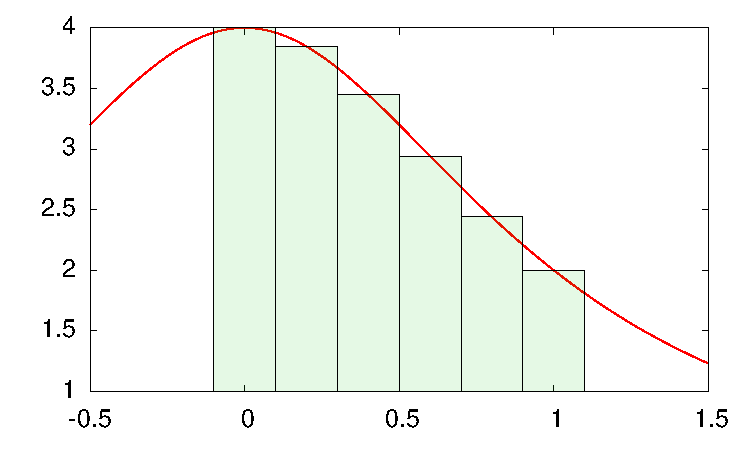
\includegraphics[width=\textwidth]{figures/integrate}\\
  6 points : $\pi \approx 3.1124$
\end{frame}
\begin{frame}
  \frametitle{Compute $\pi$ by Integration}
  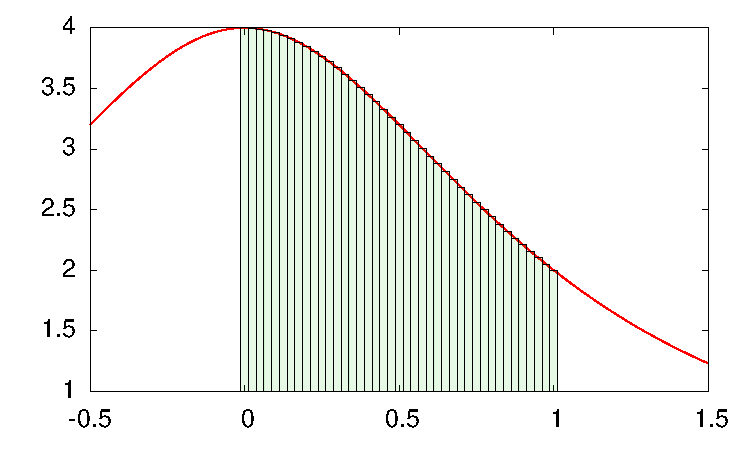
\includegraphics[width=\textwidth]{figures/integrate2}\\
  41 points : $\pi \approx 3.1380$; $10^9$ points : $\pi \approx 3.14159265$
\end{frame}

\begin{frame}[fragile]
  \frametitle{Compute $\pi$ in {\tt C++} and {\tt Fortran 90}}
  \begin{columns}[T]
    \begin{column}{0.5\textwidth}
  \begin{lstlisting}[language=C++,basicstyle=\scriptsize]
#include <iostream>
using namespace std;

double arc(double x);
const long int num_steps=1000000000;
double step;
int main()
{
  double pi, sum=0.0;
  step=1.0/(double) num_steps;

  for (int i=0;i<=num_steps;i++)
  {
    double x=(i+0.5)*step;
    sum+= arc(x);
  }
  pi = sum*step;

  cout.precision(10);
  cout << "pi is probably " 
    << fixed << pi << endl;

  return 0;
}
double arc(double x)
{
  double y = 4.0/(1+x*x);
  return y;
}
  \end{lstlisting}
\end{column}
\begin{column}{0.5\textwidth}
  \begin{lstlisting}[language=Fortran,basicstyle=\scriptsize]
program integratePi

  implicit none
  integer(kind=8) :: num_steps,i
  real(kind=8) :: sum,step,pi,x

  num_steps=1000000000
  sum=0.d0
  step=1.d0/num_steps

  do i=1,num_steps
    x=(i+0.5d0)*step
    sum=sum+arc(x)
  enddo

  pi=sum*step

  write(6, &
   '("pi is probably ",f12.10)') &
    pi

  contains
    function arc(x)
      implicit none
      real(kind=8) :: arc,x
      arc = 4.d0/(1.d0+x*x)
    end function arc
end program integratePi
  \end{lstlisting}
\end{column}
\end{columns}
\end{frame}

\begin{frame}[fragile]
  \frametitle{Compute $\pi$}
  \begin{verbatim}
>cp -r /home/sam/training/openmp/basic .
>cd pi
>module load gcc/4.5

#Compile in C++
>CXX pi.cpp -o pi
#Compile in Fortran 90
>FC pi.f90 -o pi

>qsub pi-serial.job
>cat pi.out
pi is probably 3.1415926556

real    0m25.604s
user    0m25.594s
sys     0m0.000s
  \end{verbatim}
\end{frame}

\begin{frame}
  \frametitle{Variable Scopes}
  \begin{itemize}
    \itemsep 0.5cm
    \item Scope is the lexical context which determines the lifetime of a variable
    \item In {\tt C++} variables declared in the following regions are ``locally'' scoped
      \begin{itemize}
	\item Regions in curly braces
	\item Loops
	\item Subroutines
      \end{itemize}
    \item {\tt Fortran} variables are valid within an entire subroutine and {\tt contained} subroutines and functions
    \item Global variables exist in both languages
      \begin{itemize}
	\item Variables declared as public in classes or outside of {\tt main} in {\tt C++}
	\item Common blocks or modules in Fortran
      \end{itemize}
  \end{itemize}
\end{frame}

\begin{frame}
  \frametitle{Variable Scopes}
  \begin{itemize}
    \itemsep 0.5cm
    \item \emph{lexical scope}
      \begin{itemize}
	\item The physical text where a variable is valid
      \end{itemize}
    \item \emph{dynamical scope}
      \begin{itemize}
	\item The runtime scope of a variable
      \end{itemize}
    \item Scopes will be extremely important to OpenMP
      \begin{itemize}
	\item Several clauses exist to control the scoping behavior
      \end{itemize}
  \end{itemize}
\end{frame}

\begin{frame}[fragile]
  \frametitle{Variable Scopes}
  \begin{columns}
    \begin{column}{0.5\textwidth}
  \begin{lstlisting}[language=C++,basicstyle=\scriptsize]
#include <iostream>
using namespace std;

double arc(double x);
const long int num_steps=1000000000;
double step;
int main()
{
  double pi, sum=0.0;
  step=1.0/(double) num_steps;

  for (int i=0;i<=num_steps;i++)
  {
    double x=(i+0.5)*step;
    sum+= arc(x);
  }
  pi = sum*step;

  cout.precision(10);
  cout << "pi is probably " 
    << fixed << pi << endl;

  return 0;
}
double arc(double x)
{
  double y = 4.0/(1+x*x);
  return y;
}
  \end{lstlisting}
\end{column}
\begin{column}{0.5\textwidth}
  \begin{itemize}
    \itemsep 0.3cm
    \item {\color{blue}{\tt num\_steps} and {\tt step} are global}
    \item {\color{green}{\tt pi}, {\tt step} and {\tt sum} are valid for all of {\tt main}}
    \item {\color{red}{\tt i} and {\tt x} are valid only within the {\tt for} loop}
    %\item {\color{gold}The dynamic extent of {\tt y} is in the {\tt for} loop}
  \end{itemize}
  %these values are relative to this column
  \begin{tikzpicture}[overlay]
    \draw[color=blue] (-6.3,-2.3) rectangle (-0.7,5.2);
    \draw[color=green] (-6.2,-0.85) rectangle (-0.9,3.7);
    \draw[color=red] (-6.0,1.38) rectangle (-1.2,2.85);
    %\draw[color=gold] (-6.1,-2.2) rectangle (-1.2,-0.85);
  \end{tikzpicture}
\end{column}
\end{columns}
\end{frame}

\begin{frame}[fragile]
  \frametitle{Variable Scopes}
  \begin{columns}
    \begin{column}{0.5\textwidth}
  \begin{lstlisting}[language=Fortran,basicstyle=\scriptsize]
program integratePi

  implicit none
  integer(kind=8) :: num_steps,i
  real(kind=8) :: sum,step,pi,x

  num_steps=1000000000
  sum=0.d0
  step=1.d0/num_steps

  do i=1,num_steps
    x=(i+0.5d0)*step
    sum=sum+arc(x)
  enddo

  pi=sum*step

  write(6, &
   '("pi is probably ",f12.10)') &
    pi

  contains
    function arc(x)
      implicit none
      real(kind=8) :: arc,x
      arc = 4.d0/(1.d0+x*x)
    end function arc
end program integratePi
  \end{lstlisting}
\end{column}
\begin{column}{0.5\textwidth}
  \begin{itemize}
    \itemsep 0.3cm
    \item {\color{blue}All variables declared in {\tt program} are available to {\tt arc}}
    \item {\color{red}Variables in {\tt function arc} are private to {\tt arc}}
  \end{itemize}
  %these values are relative to this column
  \begin{tikzpicture}[overlay]
    \draw[color=blue] (-6.3,-2.65) rectangle (-0.7,5.3);
    \draw[color=red] (-5.8,-2.35) rectangle (-1.1,-1.0);
  \end{tikzpicture}
\end{column}
\end{columns}
\end{frame}


\begin{frame}[fragile]
  \frametitle{Loop parallelization}
  \begin{itemize}
    \item The {\tt omp parallel for} region
      \begin{itemize}
	\item Reads the loop bounds and divides the work
	\item {\tt i} becomes private to each thread in {\tt Fortran} and {\tt C++}
	\item What other scopes do we expect?
      \end{itemize}
  \end{itemize}
  \begin{columns}[T]
    \begin{column}{0.5\textwidth}
  \begin{lstlisting}[language=C++,basicstyle=\footnotesize]
#pragma omp parallel for
  for (int i=0;i<=num_steps;i++)
  {
    double x=(i+0.5)*step;
    sum+= arc(x);
  }
  \end{lstlisting}
  {\footnotesize The locally scoped variable {\tt x} becomes private to each thread by default}
\end{column}
\begin{column}{0.5\textwidth}
  \begin{lstlisting}[language=Fortran,basicstyle=\footnotesize]
  !$omp parallel do
  do i=1,num_steps
    x=(i+0.5d0)*step
    sum=sum+arc(x)
  enddo
  !$omp end parallel do
  \end{lstlisting}
  {\footnotesize All variables except {\tt i} are shared by default}
\end{column}
\end{columns}
\end{frame}

\begin{frame}
  \frametitle{{\tt parallel} clauses}
  \begin{itemize}
    \item Scoping clauses restricted to the lexical extent
      \begin{itemize}
	\itemsep 0.5cm
	\item {\tt private (list)}
	  \begin{itemize}
	    \item Independent variables are created for each thread
	  \end{itemize}
	\item {\tt shared (list)}
	  \begin{itemize}
	    \item Can be used for reading and writing by multiple threads
	  \end{itemize}
	\item {\tt reduction (operator:variable)}
	  \begin{itemize}
	    \item A private copy is made for each thread and the reduction operator is applied at the end of the parallel region
	    \item Operators: {\tt +, *, -, \&, |, \textasciicircum, \&\&, ||}
	  \end{itemize}
	\item {\tt default (private|shared|none)}
	  \begin{itemize}
	    \item By default all variables are shared
	    \item Locally scoped variables in {\tt C++} are private
	  \end{itemize}
      \end{itemize}
  \end{itemize}
\end{frame}

\begin{frame}[fragile]
  \frametitle{Compute $\pi$ in {\tt C++} and {\tt Fortran 90} in parallel}
  \begin{lstlisting}[language=C++,basicstyle=\scriptsize]
#pragma omp parallel for reduction(+:sum)
  for (int i=0;i<=num_steps;i++)
  {
    double x=(i+0.5)*step;
    sum+= arc(x);
  }
  \end{lstlisting}
  \begin{lstlisting}[language=Fortran,basicstyle=\scriptsize]
  !$omp parallel do reduction(+:sum) &
  !$omp private(x)
  do i=1,num_steps
    x=(i+0.5d0)*step
    sum=sum+arc(x)
  enddo
  !$omp end parallel do
  \end{lstlisting}
\end{frame}


\begin{frame}[fragile]
  \frametitle{{\tt parallel for} region}
  \begin{verbatim}
>#edit and compile 
>qsub pi-parallel.job
>cat pi.out
pi is probably 3.1415926556

real    0m6.458s
user    0m25.601s
sys     0m0.005s
  \end{verbatim}
\end{frame}

\begin{frame}
  \frametitle{Loop parallelization}
  \begin{itemize}
    \item Loops that can be parallelized will have the following
      \begin{itemize}
	\itemsep 0.5cm
	\item All assignments are made to arrays
	\item Each element is assigned by at most one iteration
	\item No iteration reads elements assigned by another iteration
	\item Blocks must have one entrance and exit
      \end{itemize}
  \end{itemize}
\end{frame}


\begin{frame}
  \frametitle{Loop parallelization}
  \begin{itemize}
    \itemsep 0.5cm
    \item Loops with data dependence cannot be parallelized
      \begin{itemize}
	\item {\tt a[i] = x*a[i-1]}
	\item Data dependence exists through the \emph{dynamical} extent of a parallel region
      \end{itemize}
    \item Loops with an undefined number of iteration cannot be parallelized
      \begin{itemize}
	\item {\tt while(!converged)}
      \end{itemize}
    \item Race conditions
      \begin{itemize}
	\item {\tt sum=sum+i}
	\item Many can be cured with the {\tt reduction} clause
	%\item {\tt threadprivate} should be used with global variables and objects
      \end{itemize}
    \item Use control statements and divergent iterations carefully
      \begin{itemize}
	\item {\tt goto} must be within the block
	\item {\tt break, continue} must be within the block
	\item {\tt stop} and {\tt exit} are allowed
      \end{itemize}
  \end{itemize}
\end{frame}

\begin{frame}[fragile]
  \frametitle{Loop nesting}
  \begin{itemize}
    \item In nested loops, both loops cannot be parallel
      \begin{itemize}
	\item The inner loop would not be computed in parallel since all of the threads are already used in the outer loop
      \end{itemize}
  \end{itemize}
  \begin{lstlisting}[language=C++]
 for(int y=0; y<25; ++y)
 {
   for(int x=0; x<80; ++x)
   {
     a[y] += b[x];
   }
 }
  \end{lstlisting}
  \begin{itemize}
    \item In this example only the outer loop can be parallelized due to data dependence of {\tt a[y]}
  \end{itemize}
\end{frame}



\title{Exercises}
\author{}
\date{}
\frame{\titlepage}

\begin{frame}[fragile]
  \frametitle{Loop parallelization}
  \begin{itemize}
    \item Copy {\tt /home/sam/training/openmp/basic/}
    \item Parallelize the loops in {\tt laplace2d}, {\tt matrixvector}
  \end{itemize}
\end{frame}

\begin{frame}
\end{frame}

\begin{frame}
  \frametitle{Jacobi Iterations\footnotemark[1]}
  \begin{itemize}
    \item Iteratively converges to correct value (e.g. Temperature), by computing new values at each point from the average of neighboring points.
  \end{itemize}
  \begin{columns}
    \begin{column}{0.25\textwidth}
      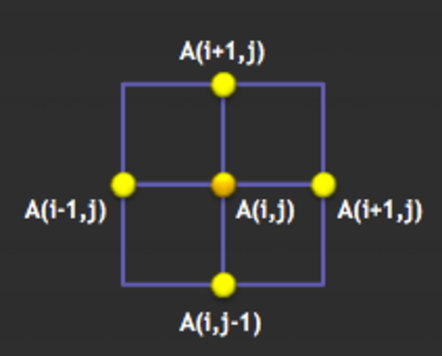
\includegraphics[width=\columnwidth]{figures/jacobi}
    \end{column}
    \begin{column}{0.75\textwidth}
      \scriptsize
      \begin{equation*}
	A_{k+1}(i,j) = \frac{A_k(i-1,j)+A_k(i+1,j)+A_k(i,j-1)+A_k(i,j+1)}{4}
      \end{equation*}
      \normalsize
    \end{column}
  \end{columns}
  \footnotetext[1]{Adapted from a recent PSC workshop}
\end{frame}


\begin{frame}[fragile]
  \frametitle{Loop parallelization}
  \begin{itemize}
    \item Parallelize the loops in {\tt matrixvector}
  \end{itemize}
      \begin{verbatim}
>cd matrixvector
>#edit mxm.c
>module purge
>module load gcc/4.5
>CXX mxm.c -fopenmp -o matrixvector
>qsub matrixvector.job
>#inspect omp.out
     \end{verbatim}
\end{frame}

\end{document}
